\section{Анализ предметной области}

В этом разделе будут проведен анализ предметной области. Описаны методы обеспечения защиты информации на современных процессорах. Дано понятие и характеристика доверенной среды исполнения.

\subsection{Кольца привилегий}

В целях безопасности, компоненты любой системы разделены на уровни привилегий -- кольца защиты, за реализацию которых отвечает разработчик процессора. Во всех современных системах, реализована кольцевая система уровней привилегий. От внешнего кольца к внутреннему идёт увеличение полномочий для инструкций кода, выполняемых на процессоре в данный момент (рис. \ref{fig:rings}).

\begin{figure}[h]
	\centering
	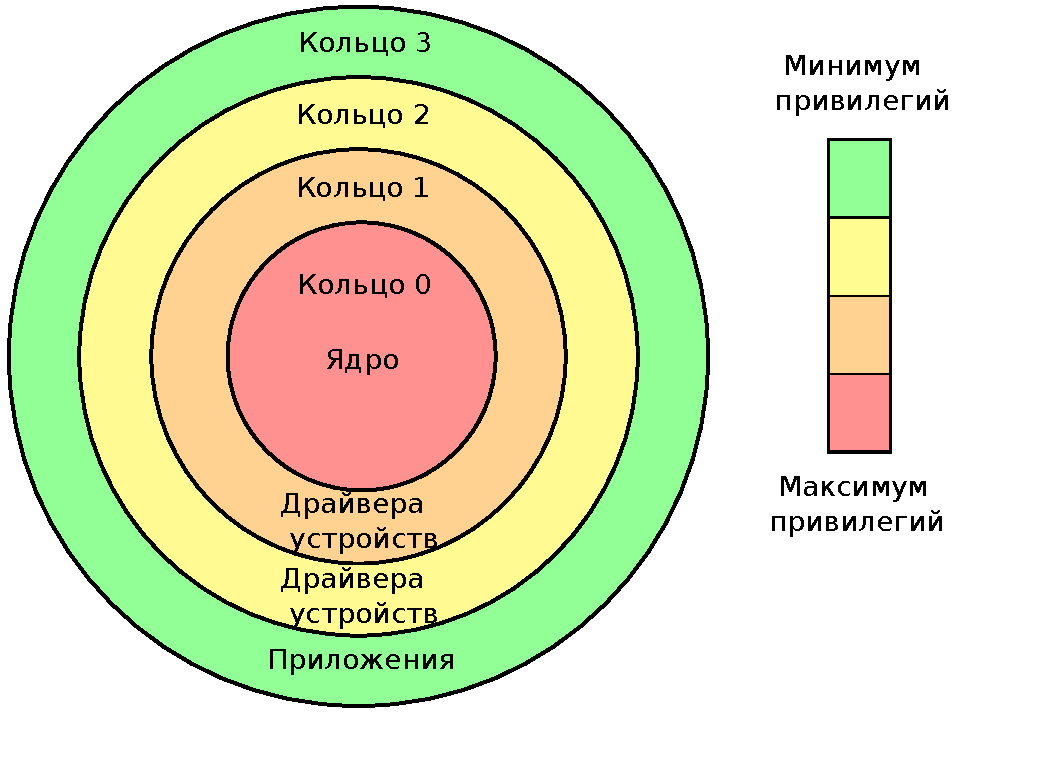
\includegraphics[width=\textwidth]{img/rings.pdf}
	\caption{Концептуальная схема представления колец защиты в современных системах}
	\label{fig:rings}
\end{figure}

Можно создавать ещё более сложную систему -- формировать ещё больше колец защиты, для ограничения каждого из компонентов системы. Однако, чем сложнее архитектура системы и чем больше количества кода в ней, тем проще злоумышленнику найти уязвимость и эксплуатировать её \cite{complex-systems}.

Главной задачей злоумышленника является получение доступ к привилегиям, которые бы позволили получить доступ к необходимым ресурсам системы. Может показаться, что архитектурно верным является решение размещать код, который отвечает за управление пользовательским данным, и конфиденциальные данные нужно исключительно на последнем кольце защиты -- ведь получить доступ туда сложнее всего. Но у такого подхода есть свои недостатки \cite{complex-systems}. Данный подход был переосмыслен -- в настоящее используется схема, когда и код, и конфиденциальные данные хранятся на одном и том же уровне, что и пользовательские предложения, однако, доступ к ним имеет только лишь процессор. Такой метод защиты информации называется анклавом или доверенной средой исполнения.

\subsection{Доверенная среда исполнения}

Доверенная среда исполнения (ДСИ) -- специальная изолированная область, предоставляющаяся процессором, которая позволяет вынести из системы часть функциональности приложений и ОС в отдельное окружение, содержимое памяти и выполняемый код в которой будут недоступны из основной системы, независимо от уровня текущих привилегий. Так, например, в ДСИ выполняется код отвечающих за реализацию различных алгоритмов шифрования, обработки закрытых ключей, паролей, процедур аутентификации и работы с конфиденциальными данными. 

В случае, если система была скомпрометирована, информация хранящаяся в ДСИ не может быть определена, и доступ к ней будет ограничен лишь внешним программным интерфейсом. В отличии от других методов защиты защиты информации, таких как например гомоморфное шифрование, аппаратная реализация ДСИ практически не влияет на производительность системы и уменьшает время разработки программного обеспечения \cite{tee}.

С другой стороны, аппаратная реализация ДСИ имеет свои недостатки:

\begin{itemize}
	\item некоторые современные процессоры имеют лишь частичную поддержку ДСИ либо не имеют её вовсе;
	\item нет возможности программно исправить уязвимость. Найденные уязвимости в реализации ДСИ могут быть исправлены лишь в новых ревизиях процессора, т.е. без его физической замены, злоумышленник сможет эксплуатировать уязвимость.
	\item увеличивается издержки производства на разработку таких процессоров -- их конечная стоимость возрастает.
\end{itemize}

Таким образом, в некоторых случаях, появляется необходимость в программной реализации ДСИ. Стоит отметить, что в конечном счёте, программная реализация всё равно использует другие аппаратные механизмы предоставляемые процессором \cite{aaa}.
 
\section{Существующие реализации ДСИ}

\subsection{Intel SGX}

Intel

\subsection{Keystone}

RISC V

\subsection{ARM TrustZone}

ARM TrustZone -- технология аппаратного обеспечения ДСИ, разрабатываемая компанией ARM. Большинство процессоров разработанных ARM имеют поддержку TrustZone \cite{comparsion-arm-intel}. Данная технология основана на разделении режимов работы процессора на два "мира": обычный мир (Normal World) и безопасный мир (Secure World). Процессор переключается в безопасный мир по запросу (с помощью специальной инструкции), при работе с конфиденциальными данными. Всё остальное время, процессор работает в режиме обычного мира. Процессоры с поддержкой данной технологии имеют способность разделять память, независимо от её типа, на ту, которая доступна только в безопасном мире, и ту, которую можно использовать в обычном мире. ARM предоставляют открытый исход программного обеспечения для поддержки данной аппаратной технологии -- ARM Trusted Firmware \cite{arm-tfa}.

\subsubsection{Обычный и безопасный мир}

Ключевой особенной ARM TrustZone является способность процессора переключаться между обычным и безопасным миром. Каждый из этих миров управляется собственной операционной системой, которые обеспечивают необходимую функциональность. Основное различие между этими ОС заключается в предоставляемых гарантия безопасности. В один момент времени, процессор может находиться только в одном из двух миров, что определяется значением специального бита NS (Non-Secure), бит является частью регистра Secure Configuration Register (SCR). Этот регистр доступен для периферии только для чтения, изменять его значение может лишь сам процессор. Когда процессор находится в обычном режиме исполнения кода, значение бита NS равно 1, и наоборот, когда процессор находится в безопасном мире, значение бита NS равно 0.

За связь между обычным и безопасным миром отвечает специальный механизм -- Secure Monitor. Он соединяет оба мира и является единственной точкой входа в безопасный мир. Для того, чтобы из обычного мира перейти в безопасный, существует специальная инструкция процессоров ARM -- Secure Monitor Call (SMC). При вызове данной инструкции процессор передает управление Secure Monitor. Тот в свою очередь готовим систему к переходу из одного мира в другой и передает управление соответствующей ОС. Инструкция SMC используется как для перехода из нормального мира в безопасный, так и для перехода из безопасного в нормальный. Некоторые прерывания или исключения могут быть настроены так, чтобы они так же проходили через Secure Monitor и были обработаны в безопасном мире. ARM предоставляет спецификацию Secure Monitor Call Calling Convention (SMCCC) \cite{smccc}, которая является стандартом при реализации вызовов SMC. 

На рисунке \ref{fig:trustzone-conceptual} представлена цонепутальная схема взаимодействия двух миров.

\begin{figure}[h]
	\centering
	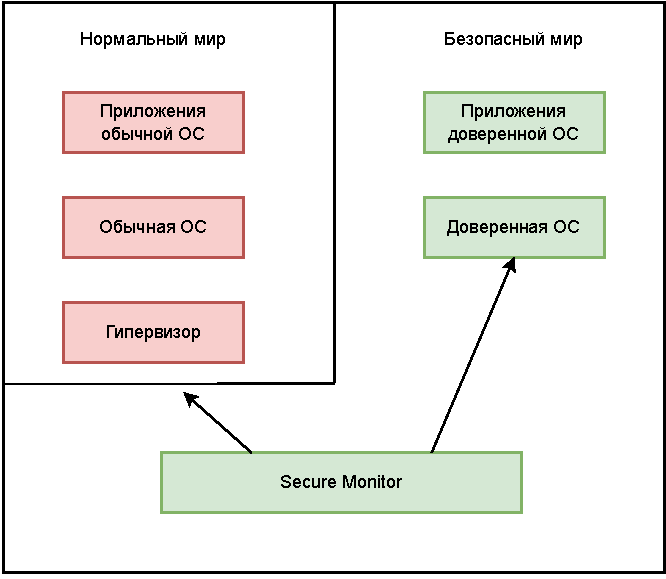
\includegraphics[width=\textwidth]{img/arm-conceptual.pdf}
	\caption{Концептуальная схема взаимодействия двух миров для процессоров ARM Cotrex-A}
	\label{fig:trustzone-conceptual}
\end{figure}

Доверенная операционная система, так же как и обычная, может запускать приложения. Они, как и в обычном мире, обращаются к доверенной ОС при необходимости получения каких-либо ресурсов или обработки прерываний и исключений. Таким образом, Secure Monitor передаёт управление одному из доверенных приложений, и уже те, в свою очередь, обращаются к доверенной ОС.

ARM предоставляют открытый исходной код эталонной доверенной операционной системы, которая называется OP-TEE \cite{optee}. Global Platform предоставляет спецификацию для реализации API взаимодействия доверенных приложений \cite{teec-spec} с доверенной ОС \cite{tee-spec}.

Физически миры разделены таким образом, что часть регистров доступны только в безопасном мире. Периферия, например память, может быть настроена так, что она может быть доступна лишь в определенном мире. Технология TrustZone в нормальном режиме работы процессора не позволяет программному обеспечению получить доступ к аппаратным средствам, которые могут быть доступны лишь только в безопасном мире. 

При сборке компонентов системы, производитель устройства должен позаботиться о конфигурации периферии для работы с TrustZone:

\begin{itemize}
	\item если предполагается, что периферия может получать доступ к безопасному режиму исполнения, процессор и внешнее устройство должны быть соединены (помимо различных шин) линией NS. Получение сигнал NS=0 от процессора к периферии означает, что команда является доверенной (например операция чтения или записи).
	\item в обратном случае, линия NS может быть опущена. Предполагается, что такая периферия не имеет никаких привилегий, т.е. NS=1 всегда.
\end{itemize}

На рисунке \ref{fig:ns-bit} представлена схема взаимодействия процессора и периферии для поддержки TrustZone. Периферийные устройства №1 и №3 соединены линией NS, а устройство №2 нет.

\begin{figure}[h]
	\centering
	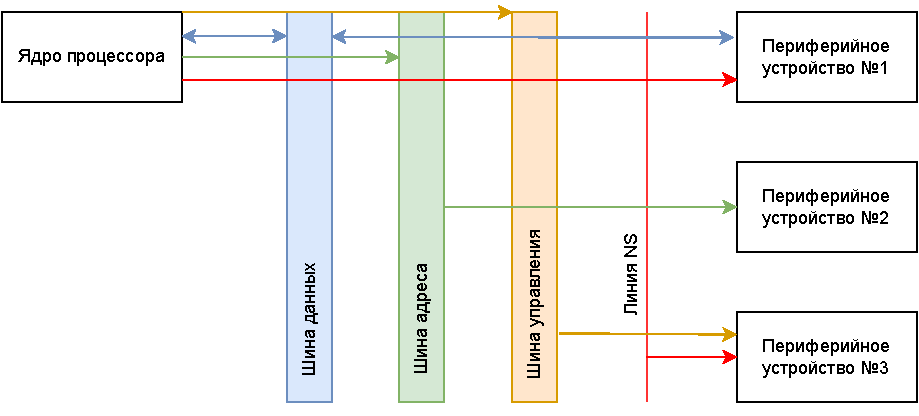
\includegraphics[width=\textwidth]{img/arm-ns.pdf}
	\caption{Пример взаимодействия процессора и периферии для поддержки TrustZone}
	\label{fig:ns-bit}
\end{figure}

Стоит отметить, что чаще всего не вся периферия соединена сигналом NS с процессором. Например, тот факт, что производитель устройства не соединил сигналом NS камеру и ядра процессора, полностью исключает возможность предоставления пользователю доступа к устройству с помощью технологии распознавания лица.

\subsubsection{Режимы работы процессора}

Современная архитектура ARM поддерживается три режима работы процессора: 

\begin{itemize}
	\item \texttt{EL0} -- непривилегированный режим работы, предназначенный для исполнения обычных программ;
	\item \texttt{EL1} -- привилегированный режим работы -- исполняется кода ОС, обработчиков прерываний и исключений;
	\item \texttt{EL2} -- режим работы гипервизора.
\end{itemize}

Для того, чтобы программа исполняемая на уровне EL0 могла перейти в EL1 (например, обратиться к ресурсам доступным только ОС), в архитектуре ARM существует команда Supervisor Call (SVC). Аналогично, команда Hypervisor Call (HVC) предназначена для перехода из режима EL1 в EL2.

Каждый из этих уровней могут исполняться в нормальных (Non-Secure) так и безопасных (Secure) режимах (рис. \ref{fig:arm-levels})

\begin{figure}[h]
	\centering
	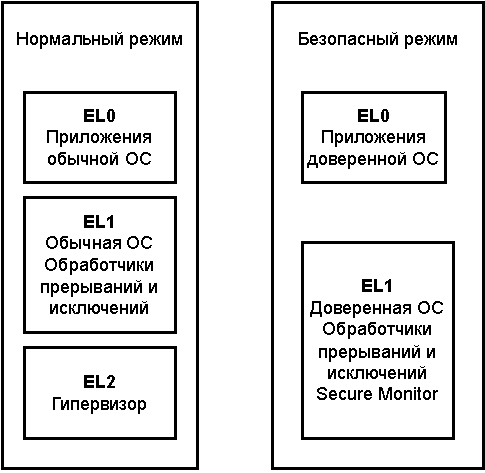
\includegraphics[width=\textwidth]{img/arm-levels.pdf}
	\caption{Режимы работы процессоров архитектуры ARM}
	\label{fig:arm-levels}
\end{figure}

\begin{itemize}
	\item обычные приложения исполняются на уровне Non-Secure EL0, а приложения доверенной ОС на Secure EL0;
	\item обычная ОС выполняется на уровне Non-Secure EL1; все прерывания и исключения произошедшие в нормальном мире так же обрабатываются на этом уровне; доверенная ОС и прерывания произошедшие в безопасном мире исполняются на уровне Secure EL1;
	\item Secure Monitor всегда исполняется на уровне Secure EL1;
	\item гипервизор исполняется в режиме Non-Secure EL2.
\end{itemize}

Бит NS, который был описан в предыдущей главе, определяет то, в каком режиме сейчас исполняется код: обычном (NS=1) или безопасном (NS=1).

Благодаря дублированию нормального и безопасного режима архитектура ARM позволяет запустить сразу две ОС: обычную и доверенную.

\subsubsection{Разделение памяти}

В целях безопасности в ARM TrustZone память разделяется на защищенную и незащищенную область. Благодаря контроллеру адресного пространства (TZASC -- TrustZone Address Space Controller) незащищенная область память может использоваться только из обычного мира, а защищенная из безопасного. Кэш память так же разделяется на защищенную и незащищенную. Необходимо отметить, что данный контролер не является обязательным в архитектуры ARM TrustZone, поэтому разработчики могут принять решение отказаться от них в пользу более компактных и менее энергоемких устройств.

\subsubsection{Проверка целостности}

Проверка целостности ДСИ является важным механизмом, который не позволит злоумышленнику изменить исходный код доверенной ОС или доверенных приложений. В ARM TrustZone данный механизм реализован на аппаратном уровне как для ОС, так и для приложений: каждый раз, при загрузке доверенной ОС в память, с помощью цифровой подписи проверяются её целостность. Аналогичная схема используется и при загрузке доверенных приложений. Запустить ОС может только подписанные приложения, подпись формируется разработчиками, на стадии компиляции в исполняемый файл.

На данный момент, доверенная среда исполнения от компании ARM не поддерживает процедуру удалённой проверенной проверки (например, с помощью сервера). Существуют лишь программные решения этой проблемы от сторонних разработчиков \cite{comparsion-arm-intel}.

\section{Сравнение реализаций ДСИ}

\subsection{Критерии сравнения}

Для сравнения раннее описанных реализаций ДСИ были выделены следующие критерии:

\begin{itemize}
	\item К1 - безопасность;
	\item K2 - производительность;
	\item К3 - надежность механизма аттестации ДСИ;
	\item К4 - наличие открытого исходного кода.
\end{itemize}

\pagebreak
